\documentclass[12pt, a4paper]{article}
\usepackage[bottom=2cm,top=3cm,left=3cm,right=2cm]{geometry}
\usepackage[brazilian]{babel} % Traduz alguns termos para o português
\usepackage[utf8]{inputenc} % Reconhece acentuação
\usepackage{color,graphicx}
\usepackage{enumerate}
\usepackage{mathtools}
\usepackage{listings}
\usepackage{longtable}
\usepackage[section]{placeins}
\usepackage[hidelinks=true]{hyperref}
\hypersetup{
	colorlinks=false,     
	urlcolor=blue
}

\definecolor{olive}{RGB}{175,128,0}
\definecolor{Aquamarine}{RGB}{0,175,175}

\usepackage{setspace}
\onehalfspacing	
\setlength{\parindent}{30pt}

\usepackage{indentfirst}

\title{
	\begin{large}
		Estudo de Caso 02: Comparação de Duas Amostras
	\end{large}	}
\author{Gustavo Vieira Costa - 2010022003\\Rafael Castro - 2013030210\\Thaís Matos Acácio - 2013030287}
\date{08/04/2016}

\begin{document}
	\maketitle
	
	\vspace*{-7.5cm}
	{\bf
		\begin{center}
			{\large
				\hspace*{0cm}Universidade Federal de Minas Gerais} \\
			\hspace*{0cm}Engenharia de Sistemas  \\
		\end{center}
	}
	\vspace*{5cm}
	
\section{Introdução}
O BMI (\textit{body mass index}, ou índice de massa corporal) é um indicador frequentemente usado em avaliações clínicas de questões relacionadas ao peso de um indivíduo. Este índice é calculado como a razão entre o peso e o quadrado da estatura.
\par O objetivo desse experimento é comparar o BMI médio de duas populações de estudantes: alunos de graduação em Engenharia de Sistemas e alunos de pós-graduação em Engenharia Elétrica, com interesse de relacionar o efeito do curso na forma física dos alunos.

\section{Coleta de dados}
Resultados a partir de uma amostra aleatória obedecem as leis de probabilidade, as quais governam o comportamento aleatório e permitem inferência confiável sobre a população.
\par A Tabela \ref{table:amostra} contém a amostra de dados coletados, informados pelos alunos de cada turma, juntamente com o valor do índice BMI calculado utilizando a seguinte fórmula:
\begin{equation}
bmi = \frac{m}{h^{2}}
\end{equation}
\newline onde \textit{m} é o peso dado em kg e \textit{h} a altura dada em metros. A distribuição do BMI, de acordo com o curso, foi exibida no gráfico de blocos \ref{fig:blocos} para possibilitar uma melhor visualização da diferença entre as amostras.
\pagebreak
\begin{longtable}{|c|c|c|c|c|}
\hline
\rule[-1.0ex]{0pt}{4.0ex}
\textbf{Curso}&\textbf{ID}&\textbf{Altura(m)}&\textbf{Peso(kg)}&\textbf{BMI}\\ \hline
\endhead
\rule[-1.0ex]{0pt}{4.0ex}
PPGEE&PG-ST1&1.83&77&22.99 \\ \hline
\rule[-1.0ex]{0pt}{4.0ex}
PPGEE&PG-ST2&1.67&56&20.08 \\ \hline
\rule[-1.0ex]{0pt}{4.0ex}
PPGEE&PG-ST3&1.88&86&24.33 \\ \hline
\rule[-1.0ex]{0pt}{4.0ex}
PPGEE&PG-ST4&1.77&78&24.90 \\ \hline
\rule[-1.0ex]{0pt}{4.0ex}
PPGEE&PG-ST5&1.74&78&25.76 \\ \hline
\rule[-1.0ex]{0pt}{4.0ex}
PPGEE&PG-ST6&1.98&113&28.82 \\ \hline
\rule[-1.0ex]{0pt}{4.0ex}
PPGEE&PG-ST7&1.70&77&26.64 \\ \hline
\rule[-1.0ex]{0pt}{4.0ex}
PPGEE&PG-ST8&1.81&78&23.81 \\ \hline
\rule[-1.0ex]{0pt}{4.0ex}
PPGEE&PG-ST9&1.55&54&22.48 \\ \hline
\rule[-1.0ex]{0pt}{4.0ex}
PPGEE&PG-ST10&1.82&96&28.98 \\ \hline
\rule[-1.0ex]{0pt}{4.0ex}
PPGEE&PG-ST11&1.81&73&22.28 \\ \hline
\rule[-1.0ex]{0pt}{4.0ex}
PPGEE&PG-ST12&1.65&61&22.41 \\ \hline
\rule[-1.0ex]{0pt}{4.0ex}
PPGEE&PG-ST13&1.65&60&22.04 \\ \hline
\rule[-1.0ex]{0pt}{4.0ex}
PPGEE&PG-ST14&1.73&76&25.39 \\ \hline
\rule[-1.0ex]{0pt}{4.0ex}
PPGEE&PG-ST15&1.75&85&27.76 \\ \hline
\rule[-1.0ex]{0pt}{4.0ex}
PPGEE&PG-ST16&1.81&74&22.59 \\ \hline
\rule[-1.0ex]{0pt}{4.0ex}
PPGEE&PG-ST17&1.82&67&20.23 \\ \hline
\rule[-1.0ex]{0pt}{4.0ex}
PPGEE&PG-ST18&1.70&64&22.15 \\ \hline
\rule[-1.0ex]{0pt}{4.0ex}
PPGEE&PG-ST19&1.65&64&23.51 \\ \hline
\rule[-1.0ex]{0pt}{4.0ex}
PPGEE&PG-ST20&1.75&88&28.73 \\ \hline
\rule[-1.0ex]{0pt}{4.0ex}
PPGEE&PG-ST21&1.85&96&28.05 \\ \hline
\rule[-1.0ex]{0pt}{4.0ex}
PPGEE&PG-ST22&1.83&85&25.38 \\ \hline
\rule[-1.0ex]{0pt}{4.0ex}
PPGEE&PG-ST23&1.78&58&18.31 \\ \hline
\rule[-1.0ex]{0pt}{4.0ex}
PPGEE&PG-ST24&1.70&72&24.91 \\ \hline
\rule[-1.0ex]{0pt}{4.0ex}
PPGEE&PG-ST25&1.70&65&22.49 \\ \hline
\rule[-1.0ex]{0pt}{4.0ex}
PPGEE&PG-ST26&1.72&98&33.13 \\ \hline
\rule[-1.0ex]{0pt}{4.0ex}
PPGEE&PG-ST27&1.67&53&19.00 \\ \hline
\rule[-1.0ex]{0pt}{4.0ex}
PPGEE&PG-ST28&1.79&78&24.34 \\ \hline
\rule[-1.0ex]{0pt}{4.0ex}
EngSis&ES-ST1&1.56&48&19.72 \\ \hline
\rule[-1.0ex]{0pt}{4.0ex}
EngSis&ES-ST2&1.67&61.5&22.05 \\ \hline
\rule[-1.0ex]{0pt}{4.0ex}
EngSis&ES-ST3&1.68&60&21.26 \\ \hline
\rule[-1.0ex]{0pt}{4.0ex}
EngSis&ES-ST4&1.65&63&23.14 \\ \hline
\rule[-1.0ex]{0pt}{4.0ex}
EngSis&ES-ST5&1.69&57&19.96 \\ \hline
\rule[-1.0ex]{0pt}{4.0ex}
EngSis&ES-ST6&1.83&80&23.89 \\ \hline
\rule[-1.0ex]{0pt}{4.0ex}
EngSis&ES-ST7&1.71&76&25.99 \\ \hline
\rule[-1.0ex]{0pt}{4.0ex}
EngSis&ES-ST8&1.71&70&23.94 \\ \hline
\rule[-1.0ex]{0pt}{4.0ex}
EngSis&ES-ST9&1.65&70&25.71 \\ \hline
\rule[-1.0ex]{0pt}{4.0ex}
EngSis&ES-ST10&1.83&66&19.71 \\ \hline
\rule[-1.0ex]{0pt}{4.0ex}
EngSis&ES-ST11&1.64&52&19.33 \\ \hline
\rule[-1.0ex]{0pt}{4.0ex}
EngSis&ES-ST12&1.78&68&21.46 \\ \hline
\rule[-1.0ex]{0pt}{4.0ex}
EngSis&ES-ST13&1.76&82.5&26.63 \\ \hline
\caption{Tabela de Amostras}
\label{table:amostra}
\end{longtable}
\begin{figure}[h]
\centering
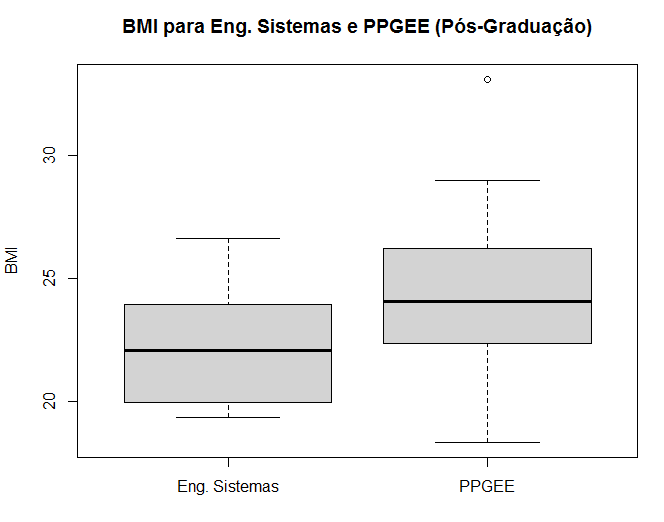
\includegraphics[scale=0.6]{img/boxplot.png}
\caption{Distribuição das amostras}
\label{fig:blocos}
\end{figure}
\par De acordo com o \textit{Teorema do Limite Central}, se a amostra tiver tamanho $n$ suficiente, a distribuição amostral de $\bar{x}$ é aproximadamente Normal. Nesse caso, iremos assumir que $n_{1}$ e $n_{2}$ são suficientes, conforme o gráfico de normalidade presente na figura \ref{fig:normal}.
\begin{figure}[h]
\centering
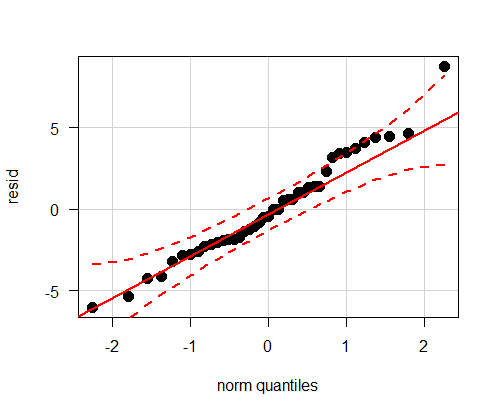
\includegraphics{img/plot-normalidade.png}
\caption{Normalidade das amostras}
\label{fig:normal}
\end{figure}

\section{Estratégia de Inferência}
\label{sec:estrategia-inferencia}
O processo de inferência estatística consiste em tirar conclusões sobre uma população com base em informações extraídas de amostras da mesma. No presente estudo de caso, os parâmetros sobre os quais temos interesse são as médias $\mu_{1}$ e $\mu_{2}$ do índice BMI das populações: alunos de graduação em Engenharia de Sistemas e alunos de pós graduação em Engenharia Elétrica.
\newline
\newline
\textbf{Hipóteses de Teste}
\par O teste estatístico é planejado para avaliar a força da evidência \textit{contra} a hipótese nula $H_{0}$. Usualmente, a hipótese nula é uma afirmativa de "nenhum efeito". A afirmativa sobre a população \textit{a favor} da qual estamos tentando achar evidência é a hipótese alternativa $H_{1}$. Logo, as hipóteses são:
\begin{equation}
\left \{
\begin{array}{cc}
H_{0}: & \mu_{1} = \mu_{2} \\
H_{1}: & \mu_{1} > \mu_{2} \\
\end{array}
\right.
\end{equation}
\newline sendo $\mu_{1}$ a média da população do PPGEE, e $\mu_{2}$ a média dos alunos de graduação em Engenharia de Sistemas.
\par Para escolha do teste estatístico que será utilizado no projeto inicialmente é preciso estudar se existe igualdade entre as variâncias das duas populações, para isso podemos utilizar o teste F assumindo como hipótese nula a igualdade de duas variâncias, portanto:
\begin{equation}
\left \{
\begin{array}{cc}
H_{0}: var_{1} = var_{2} \\
H_{1}: var_{2} = var_{1} \\
\end{array}
\right.
\end{equation}
Os resultados do teste F definem se utilizaremos o teste t para duas amostras ou o teste welch.
\newline
\textbf{Premissas do Teste}


\section{Projeto experimental}
\label{sec:projeto-experimental}

\section{Análise dos Resultados}

\section{Conclusão}

\begin{thebibliography}{7}
\bibitem{1}{\url{https://github.com/fcampelo/Design-and-Analysis-of-Experiments}}
\bibitem{2}{Estatística Aplicada e Probabilidade para Engenheiros (4ª edição) - Montgomery}
\bibitem{3}{A Estatística Básica e Sua Prática (6ª edição) - David S. Moore, William I. Nortz, Michael A. Fligner}
\bibitem{4}{\url{https://www.youtube.com/watch?v=SacXljL9dKQ&nohtml5=False}}
\bibitem{5}{\url{https://www.youtube.com/watch?v=TJbnkmiZiRU&nohtml5=False}}
\bibitem{6}{\url{https://stat.ethz.ch/R-manual/R-devel/library/stats/html/var.test.html}}
\bibitem{7}{\url{http://ww2.coastal.edu/kingw/statistics/R-tutorials/independent-t.html}}
\end{thebibliography}		
		
\end{document}